\section{Dataset}

\begin{frame}{About Dataset}

  \begin{itemize}
    \item Our data describes performance of basketball team in each season.
    \item Data from the 2013 to 2023 Division I college basketball seasons.
    \item Rows are state teams
    \item Columns contain number of games played and games won along with other features of the team
  \end{itemize}
  
\end{frame}

\begin{frame}{Parameter of Interest and Goal of Project}

  \begin{itemize}
    \item Total number of games played
    \item Total number of games won
    \item Goal: Analysis of probabilities of a team winning a game in the upcoming season
  \end{itemize}

  \vspace{0.25in}

  \begin{figure}
    \centering
    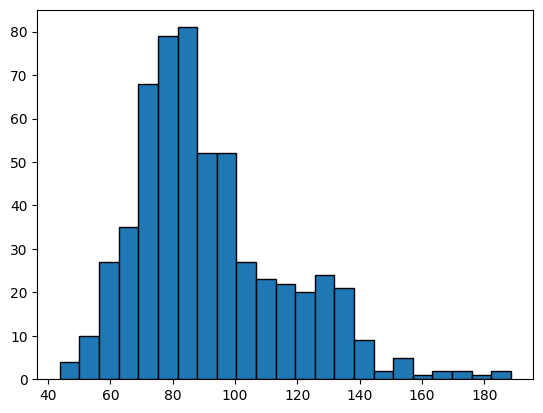
\includegraphics[width=0.5\linewidth]{../Report/images/data-hist.png}
    \caption{Histogram of Perimeter Mean}
  \end{figure}
  
\end{frame}
